\cleardoubleoddpage
\chapter{Background and Related Work}
\label{chap:background}
\begingroup
\fontsize{11pt}{13.2pt}\selectfont

This chapter provides the theoretical and empirical context for the two experimental tracks developed in this thesis. We survey the landscape of out-of-distribution (OOD) detection, covering discriminative and generative approaches and their known limitations, then review the diffusion model foundations used throughout. We further describe industrial quality classification baselines and identify the research gaps that motivate our contributions.
\section{Out-of-Distribution Detection}
\label{sec:bg:ood}

Out-of-distribution detection addresses a fundamental challenge in deploying machine learning models: identifying when test samples differ significantly from the training distribution. This section formalises the OOD detection problem, characterises different types of distribution shift, and discusses why robust OOD detection is critical for real-world applications.

\subsection{Problem Definition}
\label{sec:bg:ood:problem}

Let $\mathcal{X}$ denote the input space and $\mathcal{Y}$ denote the label space. During training, we have access to a dataset $\mathcal{D}_{\text{train}} = \{(x_i, y_i)\}_{i=1}^{n}$ drawn i.i.d.\ from an in-distribution (ID) $P_{\text{train}}(x, y)$. A model $f_\theta : \mathcal{X} \to \mathcal{Y}$ is learnt to minimise some loss function $\mathcal{L}$ over this distribution:

\begin{equation}
\label{eq:bg:loss}
\theta^* = \arg\min_\theta \; \mathbb{E}_{(x,y) \sim P_{\text{train}}} \left[ \mathcal{L}(f_\theta(x), y) \right]
\end{equation}

At test time, the model may encounter samples $x_{\text{test}}$ that come from a different distribution $P_{\text{ood}}(x)$. The goal of OOD detection is to determine whether a given test sample $x$ is drawn from $P_{\text{train}}$ or $P_{\text{ood}}$ without access to labels from the OOD distribution during training. Formally, we seek a scoring function $s : \mathcal{X} \to \mathbb{R}$ such that:

\begin{equation}
\label{eq:bg:scoring}
s(x) \begin{cases}
> \tau & \text{if } x \sim P_{\text{ood}} \\
\leq \tau & \text{if } x \sim P_{\text{train}}
\end{cases}
\end{equation}

where $\tau$ is a threshold that can be calibrated using a held-out validation set from $P_{\text{train}}$.

The effectiveness of an OOD detector is typically evaluated using metrics that assess the separability of ID and OOD scores:

\begin{itemize}
    \item \textbf{Area Under the ROC Curve (AUROC):} Measures the probability that a randomly chosen OOD sample has a higher score than a randomly chosen ID sample. An AUROC of 1.0 indicates perfect separation, while 0.5 represents random guessing.
    \item \textbf{False Positive Rate at 95\% True Positive Rate (FPR@TPR95):} Measures the fraction of ID samples incorrectly classified as OOD when the threshold is set such that 95\% of OOD samples are correctly identified. Lower values indicate better performance.
    \item \textbf{Detection Accuracy:} The proportion of correctly classified samples (both ID and OOD) when using an optimal threshold. While simple to interpret, this metric can be misleading when ID and OOD sample sizes are imbalanced.
\end{itemize}

Distribution shift can take several forms (covariate shift, label shift, or \textbf{semantic shift}), each presenting distinct challenges~\cite{yang2021generalized}. Our work primarily addresses semantic shift (test classes absent from training) with both \textbf{near-OOD} scenarios (e.g., CIFAR-100 when trained on CIFAR-10) and \textbf{far-OOD} scenarios (e.g., SVHN, Textures).

\section{Deep Learning Approaches}
\label{sec:bg:deeplearning}

The success of deep learning in representation learning has spawned numerous OOD detection methods. These can be broadly categorised into discriminative methods that exploit classifier properties and generative methods that model the data distribution.

\subsection{Discriminative Methods}
\label{sec:bg:deeplearning:discriminative}

Discriminative methods leverage trained classifiers without density modelling. Key baselines include Maximum Softmax Probability (MSP)~\cite{hendrycks2017baseline}, ODIN~\cite{liang2018enhancing} (input perturbation with temperature scaling), Mahalanobis distance in feature space~\cite{lee2018simple}, and Energy-based detection~\cite{liu2020energy}. These methods are computationally efficient but can struggle when OOD samples lie near decision boundaries.

\subsection{Reconstruction-based and Generative Approaches}
\label{sec:bg:deeplearning:reconstruction}

Reconstruction-based methods use the discrepancy between input and reconstruction as an OOD indicator. Standard autoencoders measure reconstruction error $\|x - d(e(x))\|^2$ as an anomaly score, but the assumption that autoencoders fail on OOD samples often does not hold: they can generalise to reconstruct OOD inputs well, particularly with high-dimensional latent spaces. Variational autoencoders (VAEs) suffer from both likelihood misassignment and poor reconstruction quality due to posterior collapse.

Generative models that explicitly learn $P_{\text{train}}(x)$ should in principle use likelihood for OOD detection, but this intuition fails in practice. \textcite{nalisnick2019deep} demonstrated the likelihood paradox: deep generative models, including normalising flows with exact likelihoods, can assign higher likelihood to OOD data than ID data (e.g., flows trained on CIFAR-10 assign higher likelihood to SVHN). \textcite{kirichenko2020why} showed that likelihood decomposes into on-manifold and off-manifold components, with off-manifold volume often dominating. These findings motivated our investigation of diffusion models, whose reconstruction-based scoring sidesteps the likelihood paradox.


\section{Diffusion Models}
\label{sec:bg:diffusion}

Diffusion models have emerged as a powerful class of generative models, achieving strong benchmark results in image synthesis and other generative tasks. This section provides the mathematical foundations necessary for understanding how diffusion models can be applied to OOD detection.

\subsection{Mathematical Foundations}
\label{sec:bg:diffusion:foundations}

Diffusion models, also known as denoising diffusion probabilistic models (DDPMs)~\cite{ho2020denoising}, define a forward noising process and learn to reverse it.

\subsubsection{Forward Process}
\label{sec:bg:diffusion:forward}

The forward process gradually adds Gaussian noise to data over $T$ timesteps:

\begin{equation}
\label{eq:bg:forward1}
q(x_t \mid x_{t-1}) = \mathcal{N}(x_t; \sqrt{1 - \beta_t}\, x_{t-1}, \beta_t \mathbf{I})
\end{equation}

where $\{\beta_t\}_{t=1}^{T}$ is a variance schedule. Crucially, we can sample $x_t$ directly from $x_0$:

\begin{equation}
\label{eq:bg:forward2}
q(x_t \mid x_0) = \mathcal{N}(x_t; \sqrt{\bar{\alpha}_t}\, x_0, (1 - \bar{\alpha}_t)\mathbf{I})
\end{equation}

where $\alpha_t = 1 - \beta_t$ and $\bar{\alpha}_t = \prod_{s=1}^{t} \alpha_s$. As $t \to T$, $x_T$ approaches pure Gaussian noise.

\subsubsection{Reverse Process}
\label{sec:bg:diffusion:reverse}

The reverse process learns to denoise:

\begin{equation}
\label{eq:bg:reverse1}
p_\theta(x_{t-1} \mid x_t) = \mathcal{N}(x_{t-1}; \mu_\theta(x_t, t), \Sigma_\theta(x_t, t))
\end{equation}

The mean $\mu_\theta$ can be parameterised in various ways. Following DDPM, we typically predict the noise $\epsilon_\theta(x_t, t)$ and compute:

\begin{equation}
\label{eq:bg:reverse2}
\mu_\theta(x_t, t) = \frac{1}{\sqrt{\alpha_t}} \left( x_t - \frac{1 - \alpha_t}{\sqrt{1 - \bar{\alpha}_t}} \epsilon_\theta(x_t, t) \right)
\end{equation}

\subsubsection{Training Objective}
\label{sec:bg:diffusion:training}

The model is trained by minimising the variational lower bound, which simplifies to:

\begin{equation}
\label{eq:bg:training}
\mathcal{L} = \mathbb{E}_{t, x_0, \epsilon} \left[ \left\| \epsilon - \epsilon_\theta\!\left( \sqrt{\bar{\alpha}_t}\, x_0 + \sqrt{1 - \bar{\alpha}_t}\, \epsilon, \, t \right) \right\|^2 \right]
\end{equation}

where $\epsilon \sim \mathcal{N}(0, \mathbf{I})$ and $t \sim \text{Uniform}(\{1, \ldots, T\})$.

This objective has an elegant interpretation: the model learns to predict the noise that was added to clean data $x_0$ at timestep $t$.

\subsection{DDPM Variants and Extensions}
\label{sec:bg:diffusion:variants}

\textbf{Noise Schedules:} The variance schedule $\{\beta_t\}$ significantly impacts performance; cosine schedules~\cite{nichol2021improved} maintain more information at higher timesteps than linear schedules.

\textbf{Score-based Formulation:} \textcite{song2021score} showed that diffusion models learn the score function $\nabla_x \log p(x)$, revealing the connection $\epsilon_\theta(x_t, t) \approx -\sqrt{1 - \bar{\alpha}_t}\, \nabla_{x_t} \log p(x_t)$. This perspective connects diffusion models to Langevin dynamics and enables continuous-time stochastic differential equation (SDE) formulations. Accelerated samplers such as Denoising Diffusion Implicit Models (DDIM)~\cite{song2021denoising} allow fewer-step generation without retraining. This thesis uses the discrete DDPM formulation throughout.

\subsection{Conditional Diffusion Models}
\label{sec:bg:diffusion:conditional}

Conditioning enables diffusion models to generate samples from specific categories or with desired attributes.

\subsubsection{Classifier Guidance}
\label{sec:bg:diffusion:classifier-guidance}

\textcite{dhariwal2021diffusion} introduced classifier guidance, which steers generation using gradients from a separately trained classifier. While effective, it requires maintaining an auxiliary classifier.

\subsubsection{Classifier-Free Guidance}
\label{sec:bg:diffusion:classifier-free}

\textcite{ho2022classifierfree} proposed classifier-free guidance, which eliminates the need for a separate classifier:

\begin{equation}
\label{eq:bg:cfg}
\tilde{\epsilon}_\theta(x_t, t, y) = \epsilon_\theta(x_t, t, \varnothing) + w \left( \epsilon_\theta(x_t, t, y) - \epsilon_\theta(x_t, t, \varnothing) \right)
\end{equation}

During training, the condition $y$ is randomly dropped with probability $p$ (typically 0.1), allowing the model to learn both conditional and unconditional predictions. This approach has become the standard for conditional generation.

\subsubsection{Class Embeddings}
\label{sec:bg:diffusion:class-embeddings}

Conditioning typically injects class information through learnt embeddings added to timestep embeddings or through cross-attention mechanisms in transformer-based architectures.

\subsubsection{Multi-Head Conditioning}
\label{sec:bg:diffusion:multi-head}

Beyond single-label conditioning, diffusion models can be conditioned on multiple heterogeneous inputs simultaneously. In our inkjet quality control application, we employ multi-head conditioning where the model receives template type (categorical), feature type (categorical), quality label (binary), and bounding box coordinates (continuous) as separate conditioning inputs, each encoded through dedicated embedding layers before being combined. This multi-head approach enables a single model to handle diverse feature types and spatial contexts.

Diffusion models have achieved strong results across image generation, super-resolution, inpainting, and text-to-image synthesis~\cite{dhariwal2021diffusion, rombach2022highresolution}. However, their application to discriminative tasks like OOD detection and industrial quality classification remains relatively unexplored. A preliminary attempt to apply text-conditioned Stable Diffusion~\cite{rombach2022highresolution} to the inkjet defect dataset yielded unsatisfactory generation quality on this small, domain-specific dataset: the model could not reliably reproduce fine-grained defect patterns from text prompts alone, and the classification stage was never reached. This negative result motivated the shift to class-label conditioning on a lightweight binary CDM trained from scratch, which forms the basis of this work.

\subsection{Concurrent Diffusion-Based OOD Detection}
\label{sec:bg:diffusion:concurrent}

Several concurrent works explore diffusion models for OOD detection and anomaly scoring, each with a distinct mechanism. Understanding how this thesis differs from these approaches is essential for positioning the separation-loss contribution.

\textbf{Graham et al.\ (2023)} \cite{graham2023denoising} demonstrate that reconstruction error from a pre-trained unconditional diffusion model can serve as an anomaly score for medical images, noising a test input to an intermediate timestep and measuring the residual after denoising. Their method requires no class conditioning and no contrastive scoring; the OOD signal is the absolute reconstruction magnitude rather than a class-conditional difference. This thesis differs in two ways: we use \emph{binary} class-conditional denoising (airplane vs.\ non-airplane) and a \emph{contrastive} score $e_0 - e_1$ rather than absolute reconstruction error, which our ablation (Section~\ref{sec:results:ablations}) shows is essential, since absolute ID error collapses to 20.2\% AUROC on SVHN.

\textbf{DiffGuard} (Gao et al., 2023) \cite{gao2023diffguard} use a pre-trained Stable Diffusion model to measure semantic mismatch between a test image and a text description of the in-distribution class; the OOD score is the CLIP-space residual between the input and its diffusion-guided reconstruction. DiffGuard therefore relies on large-scale pre-training and text conditioning rather than task-specific binary training. In contrast, the binary CDM in this thesis is trained from scratch on a binary classification task and introduces the separation loss to \emph{explicitly} widen the reconstruction gap during training rather than measuring it post-hoc.

\textbf{Livernoche et al.\ (2024)} \cite{livernoche2024diffusion} investigate diffusion-based density estimation for anomaly detection, finding that diffusion-model likelihoods (approximated via the ELBO) can be competitive with flow-based likelihoods when properly normalised. Their study is complementary to this work: they focus on likelihood estimation, whereas we focus on reconstruction-error contrast and demonstrate that the training objective (separation loss) dominates the scoring signal. Their negative findings on raw likelihood further motivate the reconstruction-error contrastive approach taken here.

\textbf{Wu et al.\ (2024)} \cite{wu2024diffusion} show that a diffusion model's noise-prediction network is implicitly a noise classifier and that adding a contrastive training objective in noise-prediction space improves both generation and OOD discrimination. This is the closest prior work to the separation loss proposed in Chapter~\ref{chap:methodology}: both operate on noise-prediction differences under competing conditions. The key differences are scope and evaluation: Wu et al.\ study the contrastive objective as a training regulariser for generation quality, while this thesis isolates it as the primary OOD detection lever via a systematic $\lambda$ ablation, and further tests its transfer to an industrial domain.

Table~\ref{tab:bg:concurrent} summarises the key design choices across these works and this thesis.

\begin{table}[htbp]
  \centering
  \caption{Comparison of concurrent diffusion-based OOD detection methods.
    CFG = classifier-free guidance; $\checkmark$ = feature present;
    $\times$ = feature absent. ``Benchmark protocol'' refers to the
    headline evaluation setup; ``OOD type'' indicates whether the method
    was primarily evaluated on near-OOD (semantic shift), far-OOD
    (low-level statistic shift), or domain-specific anomaly inputs.}
  \label{tab:bg:concurrent}
  \scriptsize
  \setlength{\tabcolsep}{4pt}
  \begin{tabular}{@{}p{2.0cm}p{1.5cm}p{2.0cm}cc p{2.4cm} p{1.6cm}@{}}
    \toprule
    Method & Training & Scoring & \shortstack{Class\\cond.} & \shortstack{Sep.\\loss} & Benchmark protocol & OOD type \\
    \midrule
    Graham et al.\ 2023 \cite{graham2023denoising}  & Pre-trained & Abs.\ reconstruction & $\times$ & $\times$ & Medical anomaly (BraTS, CXR) & Domain-specific \\
    DiffGuard 2023 \cite{gao2023diffguard}           & Pre-trained & CLIP residual        & Text (CFG) & $\times$ & ImageNet near/far-OOD & Near + far \\
    Livernoche et al.\ 2024 \cite{livernoche2024diffusion} & From scratch & Likelihood (ELBO) & $\times$ & $\times$ & CIFAR-10 vs.\ SVHN, CelebA & Far-OOD \\
    Wu et al.\ 2024 \cite{wu2024diffusion}           & From scratch & Contrastive noise    & $\checkmark$ & $\checkmark$ & CIFAR-10/100 multi-class & Near + far \\
    \textbf{This work}                               & From scratch & Contrastive diff.\ score & Binary & $\checkmark$ & CIFAR-10 airplane-vs-rest + 5 ext.\ sets & Near + far \\
    \bottomrule
  \end{tabular}
\end{table}


\section{Low-Dimensional Data Geometry}
\label{sec:bg:manifold}

The low-dimensional concentration view posits that high-dimensional data concentrate on or near lower-dimensional structures embedded in the ambient space ($d \ll D$; for CIFAR-10, $D = 3072$ while intrinsic dimension is typically in the tens to low hundreds~\cite{pope2021intrinsic}). This view has direct implications for OOD detection.

Different generative models capture manifold structure differently: VAEs parameterise it via a latent space, flows compute exact likelihood but conflate manifold density with ambient volume (explaining the likelihood paradox), and diffusion models iteratively project noisy samples onto the learnt manifold through progressive denoising.

The manifold perspective explains why likelihood-based OOD detection fails (volume dominates distance in high dimensions) and suggests reconstruction error as an alternative: the distance from a sample to the learnt manifold provides a more reliable OOD signal than density. Diffusion models' iterative denoising can be interpreted as progressive projection onto the data manifold, where high reconstruction error indicates that a sample lies far from the learnt manifold. This perspective motivates our use of reconstruction error from conditional diffusion models as an OOD detection signal.


\section{Industrial Quality Control and Anomaly Detection}
\label{sec:bg:industrial}

As a practical application domain for the principles developed in this thesis, we investigate automated quality classification for inkjet print samples. This section reviews the relevant background on industrial visual inspection, object detection for region-of-interest extraction, and anomaly detection methods used as baselines.

\subsection{Automated Visual Inspection}
\label{sec:bg:industrial:avi}

Automated visual inspection (AVI) has become essential in modern manufacturing, replacing subjective human assessment with consistent, quantitative evaluation. In inkjet print samples, quality defects manifest as misaligned features, irregular edge roughness, incorrect spacing, and malformed dot patterns. These defects reduce production yield and compromise the feedback loop used to optimise printing parameters.

Traditional AVI systems rely on hand-crafted features and template matching, which require significant domain expertise and are brittle to variations in printing conditions. Deep learning-based approaches have largely superseded these methods, leveraging learnt representations to capture subtle quality variations that resist manual feature engineering.

A key challenge in industrial quality classification is choosing the input representation. Full-image approaches preserve global spatial context (the position of features relative to page edges and other features), while crop-based approaches focus local analysis on individual regions of interest. The retained public inkjet experiments in this thesis evaluate the crop-based YOLO+CDM path; broader full-image versus crop comparisons are left outside the retained evidence base unless released with public code, splits, and results.

\subsection{Object Detection for Feature Extraction}
\label{sec:bg:industrial:object-detection}

Modern object detection architectures, particularly the YOLO (You Only Look Once) family~\cite{redmon2016you}, enable real-time detection and localisation of objects in images. In our pipeline, we use YOLOv8~\cite{jocher2023ultralytics} to detect and extract individual printed features from full template images before quality classification.

\subsubsection{YOLOv8 Architecture}
\label{sec:bg:industrial:yolov8}

YOLOv8 uses a CSPDarknet backbone with a Feature Pyramid Network (FPN) and Path Aggregation Network (PAN) for multi-scale feature fusion. The anchor-free detection head simultaneously predicts bounding box coordinates and class probabilities. The YOLOv8n (nano) variant used in our work contains approximately 3.2M parameters and achieves real-time inference.

\begin{figure}[htbp]
    \centering
    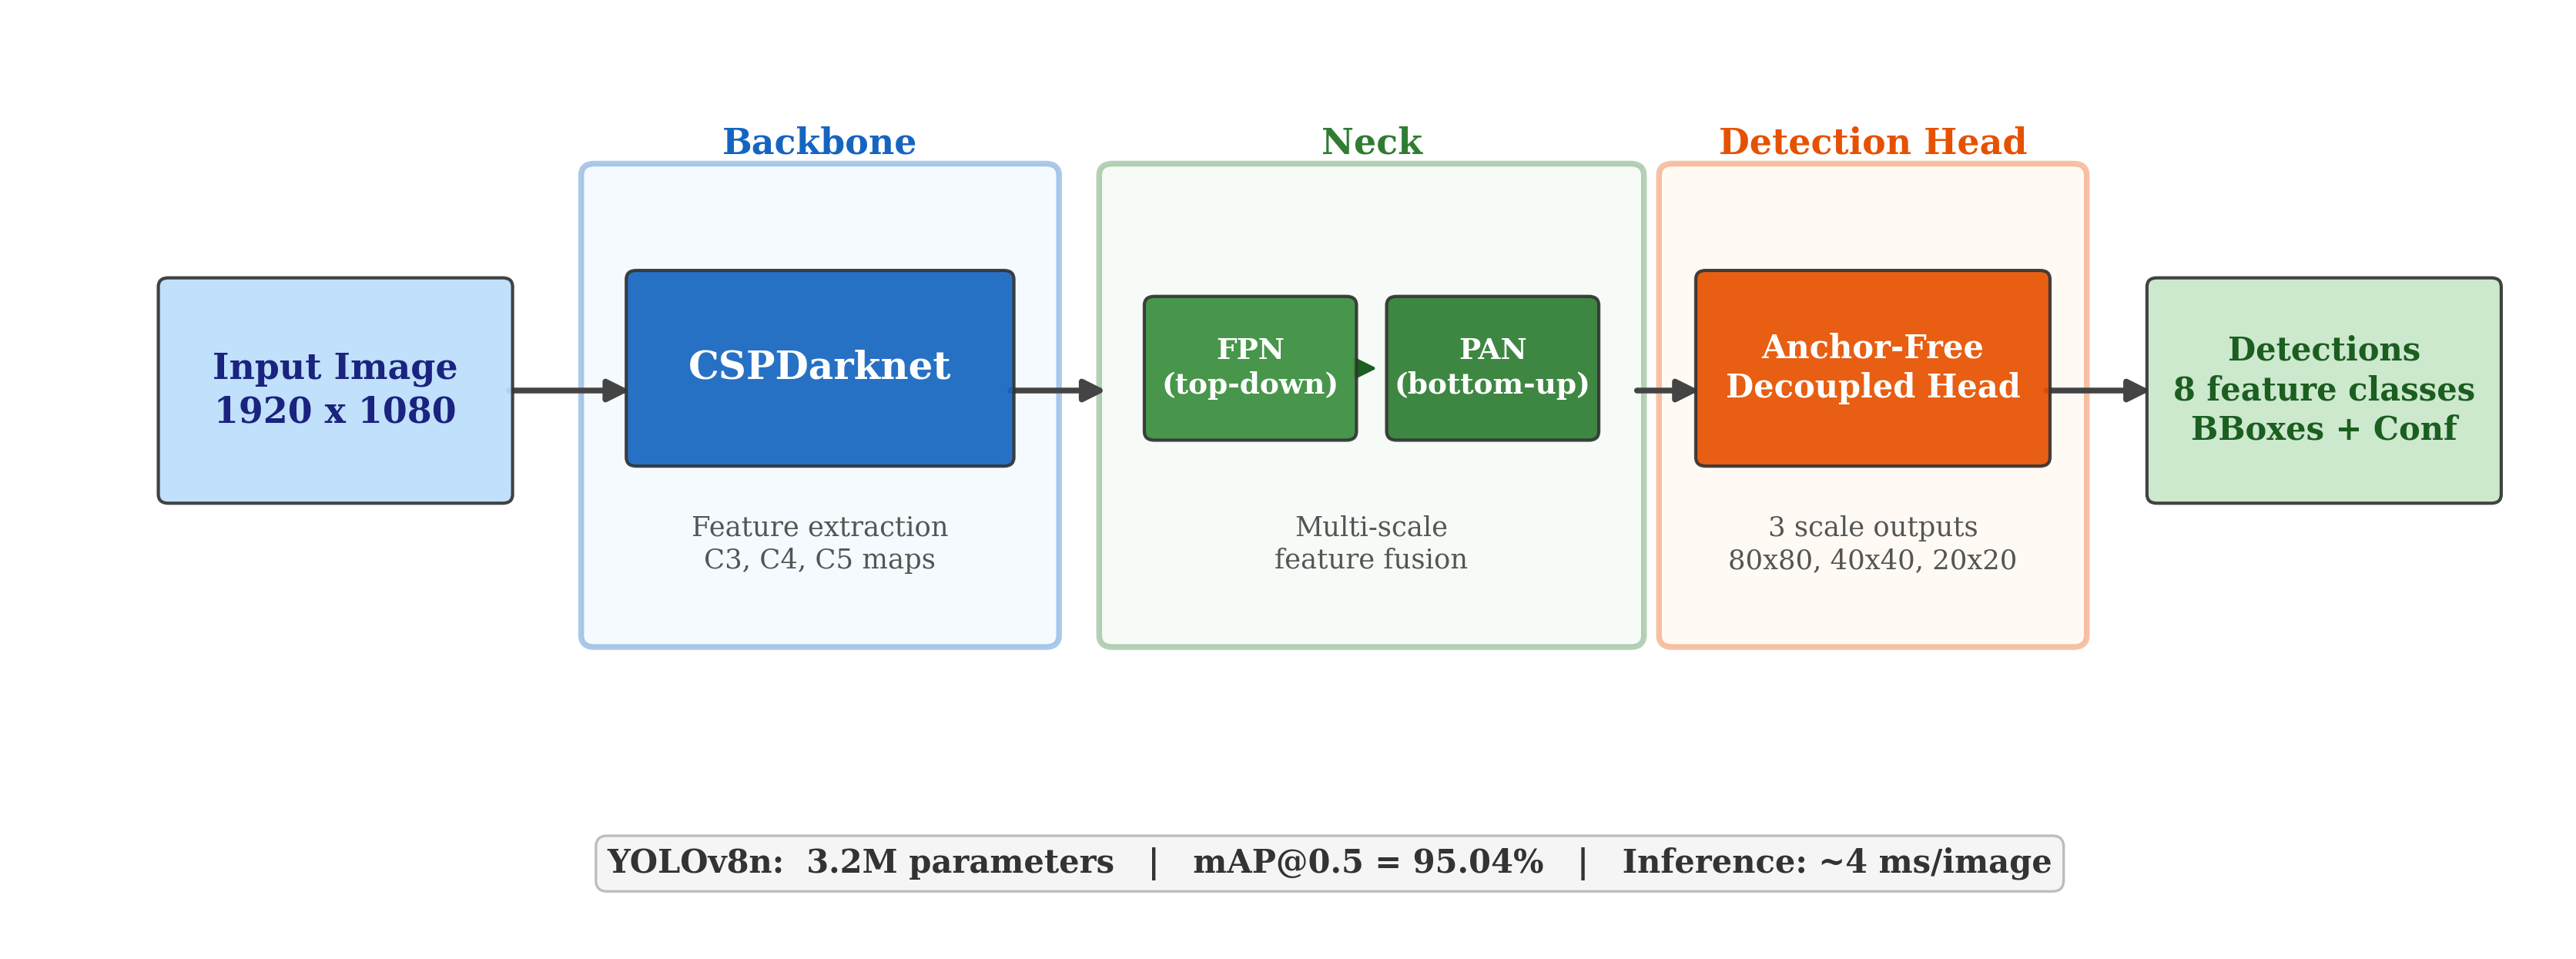
\includegraphics[width=\textwidth]{images/fig_yolov8_architecture.png}
    \caption{YOLOv8 architecture overview. The CSPDarknet backbone extracts multi-scale feature maps (C3, C4, C5), which are fused by the Feature Pyramid Network (top-down) and Path Aggregation Network (bottom-up). The anchor-free decoupled detection head produces bounding boxes, class predictions, and confidence scores at three scales. The YOLOv8n variant (3.2M parameters) achieves mAP@0.5 of 95.04\% on our inkjet feature detection task.}
    \label{fig:bg:yolov8}
\end{figure}

\subsubsection{Role in the Pipeline}
\label{sec:bg:industrial:pipeline-role}

Object detection serves as a preprocessing stage that transforms full template images ($1920 \times 1080$ pixels) into individual feature crops ($128 \times 128$ pixels). In the retained CDM evaluation, the processed source-image groups are expanded into 6{,}408 feature-level samples. Each detected region carries metadata including template type (A, B, or C), feature class (8 types), and bounding box coordinates, which serve as conditioning inputs for the diffusion model.

\subsection{Anomaly Detection Methods}
\label{sec:bg:industrial:anomaly}

Anomaly detection methods learn only from normal (defect-free) samples and detect anomalies as deviations from the learnt normality. They provide relevant context for industrial visual inspection, although non-CDM baseline experiments are not retained as thesis evidence unless they are reproducible from public artefacts.

\begin{itemize}
    \item \textbf{PatchCore}~\cite{roth2022towards}: A memory-bank approach that scores anomalies by computing the minimum distance from test patch features to a coreset of pretrained ResNet features from normal samples. Requires no training beyond feature extraction.
    \item \textbf{PaDiM}~\cite{defard2021padim}: Models normal patch features as position-wise multivariate Gaussians; anomaly scores use Mahalanobis distance from the learnt distribution.
    \item \textbf{Student-Teacher Feature Pyramid Matching (STFPM)}~\cite{wang2021studentteacher}: Knowledge distillation where a student mimics a pretrained teacher on normal data; anomalies produce feature-pyramid discrepancies.
    \item \textbf{Autoencoder:} Reconstruction-based approach where reconstruction error serves as the anomaly score, an assumption that can be unreliable for subtle quality defects.
\end{itemize}

Recent extensions include FR-PatchCore~\cite{jiang2024frpatchcore} for spatial robustness; \textcite{wang2025industrial} survey the growing application of diffusion models to industrial anomaly detection; \textcite{li2025oneformore} contribute a continual diffusion method that handles multiple anomaly types within a single model.

\subsubsection{Diffusion-Based Anomaly Detection}
\label{sec:bg:industrial:diffusion-anomaly}

A parallel line of work applies DDPM-style generative models directly to industrial anomaly detection, and is the closest antecedent to the inkjet pipeline developed in Chapter~\ref{chap:methodology}. AnoDDPM~\cite{wyatt2022anoddpm} introduced partial-diffusion anomaly scoring, noising a test image only up to an intermediate timestep and using the reconstruction residual between the original and the denoised output as the anomaly map; it demonstrated that unconditional diffusion reconstructions are competitive with feature-distance baselines on MVTec-AD without requiring any defect labels. In contrast, EfficientAD~\cite{batzner2024efficientad} takes a discriminative student--teacher route with an explicit efficiency constraint, achieving millisecond-level inference and state-of-the-art MVTec-AD numbers while using no diffusion component; it therefore serves as a strong non-diffusion reference point for the cost--accuracy trade-off discussed in Chapter~\ref{chap:discussion}. Finally, \textcite{heckler2024mvtec} release MVTec-AD 2, a substantially harder successor benchmark with real (non-synthetic) defects and multiple lighting conditions; they show that several top methods on the original MVTec-AD lose a large fraction of their AUROC when moved to MVTec-AD 2, highlighting that headline anomaly-detection numbers are benchmark-specific. Our binary CDM differs from all three: it is explicitly conditioned on a binary class variable and trained with a separation loss (Equation~\ref{eq:meth:lsep} in Chapter~\ref{chap:methodology}) rather than a purely unconditional reconstruction objective, and it produces a contrastive score across two class conditions rather than an unconditional residual.

\subsection{Supervised Classification Methods}
\label{sec:bg:industrial:supervised}

When labelled data for both good and defective samples is available, supervised classification methods provide a strong alternative. Common architectures considered in this application area include:

\begin{itemize}
    \item \textbf{ResNet-FullImg:} A standard ResNet-18~\cite{he2016deep} pretrained on ImageNet, fine-tuned on full template images resized to $224 \times 224$. This approach preserves global spatial context, allowing the model to leverage inter-feature relationships and page-level alignment cues.
    \item \textbf{ResNet-CropOnly:} The same ResNet-18 architecture applied to YOLO-cropped feature regions resized to $224 \times 224$. This isolates local feature quality but loses global context.
    \item \textbf{Dual-Branch:} Two ResNet-18 encoders process full images and cropped regions in parallel, with feature embeddings concatenated and passed through a fusion multi-layer perceptron (MLP) for final classification. A feature-type embedding provides additional conditioning.
\end{itemize}

These supervised methods serve as upper bounds for the quality classification task, establishing the achievable performance with direct label supervision.

\section{Gap Analysis and Positioning}
\label{sec:bg:gap}

We now identify gaps in the current literature and position our contributions.

\paragraph{Limitations and gaps.}
Existing likelihood-based generative OOD detectors suffer from the likelihood paradox; discriminative methods require OOD proxy data at test time. Concurrent diffusion-based OOD approaches (Section~\ref{sec:bg:diffusion:concurrent}) address the likelihood paradox via reconstruction-error scoring or pre-trained guidance, but lack systematic design studies, particularly on how training objectives and inference strategies affect AUROC in controlled settings.
Four gaps remain open: (1)~no principled study of separation-loss objectives for binary conditional diffusion OOD detection (Wu et al.~\cite{wu2024diffusion} study contrastive training for generation quality but do not ablate the separation signal as the primary OOD lever); (2)~contrastive scoring strategies are underexplored; (3)~Monte Carlo trial budgets are unstudied; and (4)~transfer conditions from large benchmarks to small industrial datasets are unknown.

\paragraph{Thesis positioning.}
\textbf{Track 1} addresses Gaps 1--3 via a binary CDM separation-loss ablation on CIFAR-10, the K-sweep, and a scoring-method comparison, all with fully public code and artefacts~\cite{DiffusionOOD}. \textbf{Track 2} addresses Gap 4: a public YOLO+CDM pipeline from \texttt{InkjetOOD}~\cite{mohammed2026inkjetood}, evaluated on the FTI\_Zer0P dataset under 5-fold cross-validation, identifies the boundary conditions under which the separation-loss gain fails to transfer.

\textbf{Practical Contribution:} We provide modular implementations built on PyTorch Lightning~\cite{falcon2019pytorch} and Hydra~\cite{yadan2019hydra} with evaluation tools, reproducibility measures, and documentation. The CIFAR-10/OOD benchmark code is publicly available at \url{https://github.com/ahmed-3m/DiffusionOOD}, with weights at \url{https://huggingface.co/ahmed-3m/DiffusionOOD}. The inkjet CDM implementation is publicly available at \url{https://github.com/ahmed-3m/InkjetOOD}~\cite{mohammed2026inkjetood}, with weights at \url{https://huggingface.co/ahmed-3m/InkjetOOD}, and uses the PROFACTOR FTI\_Zer0P dataset released on Zenodo under CC BY 4.0~\citep{profactor2024fti}.

Our work explores whether diffusion models' generative capabilities translate into discriminative signals for OOD detection and quality classification, contributing systematic ablations and practical cross-domain insights to this rapidly evolving field.
\endgroup
